\documentclass{report}
\usepackage{graphicx}
\usepackage{fancyhdr}
\usepackage{latexsym}
\usepackage{float}
\usepackage{caption}
\usepackage{amsmath}
\usepackage{geometry}
\usepackage{tikz}
\usepackage{makecell}
\usepackage{paracol}
\usepackage{lipsum}
\setlength{\parindent}{0pt}
\geometry{a4paper,scale=0.75}
%\renewcommand\thesubsection{\arabic{subsection}}
\begin{document}

    \begin{center}
        \textbf{\huge Lab Exercise \#2: Analog Output (PWM), Timers and Analog Input} \\[1em]
        Frank Li $|$
        \textbf{NetID:} jl13581 $|$
        \textbf{Email:} \texttt{jl13581@nyu.edu} $|$
        Section \textbf{C1} \\ [1em]
    \end{center}

    \begin{paracol}{2}
        {\Large \textbf{1. Background}}\\[0.5em]
        On the Playground Circuit Ciassic board, the chip using is the ATmega32U4, which has one ADC built within it. In real-worldmembedded systems, engineers are oftently required to read the analog data and convert it into digital values. In this lab session, we first generate the PWM waveform from the chip, then using the ADC port to read the converted waveform passed through the low-pass filter. ADCs operate by sampling the  signal at regular intervals and converts samples into a binary number.\\[1em]
        {\Large \textbf{2. Experimental Procedure}}\\[0.5em]
        {\Large \textbf{2.a Set up the Analog Signal}}\\[0.5em]
        After uploading the set up code to the Adafruit Circuit Playground Ciassic, I got the following output:
        \begin{figure}[H]
            \centering
            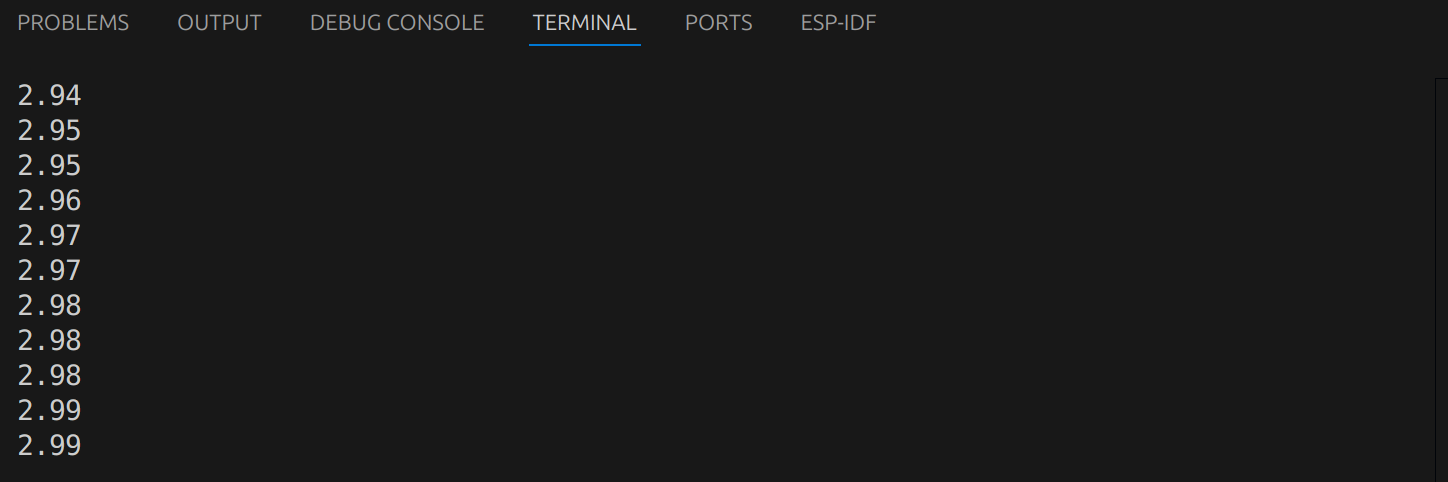
\includegraphics[width = 0.5\textwidth]{setup.png}
            \caption{Serial Output After Setup}
        \end{figure}
        which states that I hav correctly set up the device in generating the Sine wave.\\[0.5em]
        {\Large \textbf{2.a Set up the PWM Signal}}\\[0.5em]
        1. When we are setting up the output on the SCL(D3), the timer we must use is the Timer0/Counter0.\\[0.5em]
        2. Code for setting up the Fast PWM signal on the board:\\[0.5em]
        \begin{verbatim}
            // Timer Setup
            DDRD |= (1<<0);             // Set PD0 (Digital Pin 3) as output
            TCCR0A = 0b00100011;        // COM0B1:0 = 10 (non-inverting), 
                                           WGM01:00 = 11 (Fast PWM)
            TCCR0B = 0b00001011;        // WGM02 = 1 (Fast PWM with OCR0A as 
                                           TOP), CS02:00 = 011 (prescaler of 64)
            OCR0A = 124;                // Set TOP value for PWM
            OCR0B = 0;                  // Initialize duty cycle
           \end{verbatim}

    \end{paracol}
\end{document}